%%%%%%%%%%%%%%%%%%%%%%%%%%%%%%%%%%%%%%%%%
% University/School Laboratory Report
% LaTeX Template
% Version 3.1 (25/3/14)
%
% This template has been downloaded from:
% http://www.LaTeXTemplates.com
%
% Original author:
% Linux and Unix Users Group at Virginia Tech Wiki 
% (https://vtluug.org/wiki/Example_LaTeX_chem_lab_report)
%
% License:
% CC BY-NC-SA 3.0 (http://creativecommons.org/licenses/by-nc-sa/3.0/)
%
%%%%%%%%%%%%%%%%%%%%%%%%%%%%%%%%%%%%%%%%%

%----------------------------------------------------------------------------------------
%	PACKAGES AND DOCUMENT CONFIGURATIONS
%----------------------------------------------------------------------------------------

\documentclass{article}

\usepackage[version=3]{mhchem} % Package for chemical equation typesetting
\usepackage{siunitx} % Provides the \SI{}{} and \si{} command for typesetting SI units
\usepackage{graphicx} % Required for the inclusion of images
\usepackage{natbib} % Required to change bibliography style to APA
\usepackage{amsmath} % Required for some math elements 

\setlength\parindent{0pt} % Removes all indentation from paragraphs

\renewcommand{\labelenumi}{\alph{enumi}.} % Make numbering in the enumerate environment by letter rather than number (e.g. section 6)

\usepackage{xcolor}
\usepackage{soul}

\usepackage[a4paper, total={6in, 8in}, left=1in,right=1in,top=1.3in,bottom=1in, footskip=.2in]{geometry}

\definecolor{inlineBG}{HTML}{F3F3F3}  % same as GitHub Flavored Markdown
\sethlcolor{inlineBG}

\let\OldTexttt\texttt
\renewcommand{\texttt}[1]{\sethlcolor{inlineBG}{\ttfamily\hl{\mbox{#1}}}}

%\usepackage{times} % Uncomment to use the Times New Roman font

%----------------------------------------------------------------------------------------
%	DOCUMENT INFORMATION
%----------------------------------------------------------------------------------------

\title{Informatics Large Practical} % Title

\author{Lorenzo Baldini} % Author name

\date{\today} % Date for the report

\begin{document}

\maketitle % Insert the title, author and date


% If you wish to include an abstract, uncomment the lines below
% \begin{abstract}
% Abstract text
% \end{abstract}


%----------------------------------------------------------------------------------------
%	TABLE OF CONTENTS
%----------------------------------------------------------------------------------------

\tableofcontents
\pagebreak

%----------------------------------------------------------------------------------------
%	TABLE OF CONTENTS
%----------------------------------------------------------------------------------------

\section{Software Architecture Description}

In this section I will provides a description of the software architecture of the application. I will explain why I identified \textit{these classes} as being the right ones for my application. I will identify class hierarchical relationships between classes: which classes are subclasses of others?\\[1]

The UML Diagram in the following subsection will show the hierarchical relationships between the classes and provide a brief glance of the methods present in each class as well as their respective visibilities.

\subsection{Reasoning}
\label{Reasoning}
\begin{description}
\begin{itemize}
    \item App. The App class is the main entry point for the application. Here the inputs are validated and parsed, as well as static resources being initialised, such as the \texttt{HttpClient}. \\
    It initialises the loading of the data from the server, although this action is in fact delegated to the \texttt{Loader} class.
    
    \item Loader. The Loader class is responsible for the loading of the network resources. It does not do any processing of the data nor exception handling. This was decided to make its use more generalised. It uses static methods as network resources are expensive. This way, it ensures only one HTTP Client instance is created. It also contains the constants for the filenames of the resources on the server.
    
    \item Drone. The Drone class is the main functionality of the application. It represents a Drone, with a \texttt{Set} of \texttt{Sensor}s to be visited, and a \texttt{NoFlyZonesManager} (see later for both). Its unique responsibility is to generate the optimal \texttt{FlightPlan} visiting the sensors, with the limits imposed by the no-fly-zone manager. It contains appropriate methods to achieve this, while appropriately delegating related functionality to other classes when necessary.

    \item FlightPlan. The FlightPlan class represents a Drone flight plan. It is responsible for the generation of a FlightPlan object, and contains methods to convert it into a suitable string representation for the flightpath. It also provides a method to generate a \texttt{LineString} to be used in the results GeoJson.
    The main attribute is a \texttt{Deque} which represents a collection of moves. It is final, as it is unique to a FlightPlan instance, and not meant to be changed. \\
    The moves are represented by an inner class \texttt{FlighPlanComponent}. This represents a single Drone move, and includes start and end point, as well as the angle that was followed. It also includes an eventual sensor that was read during that move. It provides functionality to produce a \texttt{String} representation.
    
    \item NoFlyZonesManager. The NoFlyZonesManager is the map authority in the application. It provides a method \texttt{isLegalMove} to check whether a move is allowed. It includes a \texttt{Set} of \texttt{NoFlyZone} (see later). It includes a \texttt{final static} confinement area NoFlyZone. I chose to represent the confinement area by such object, as this provides the most generalised way of implementing all the needed functionality. By being a NoFlyZone, the confinement area can be changed easily, as well as being managed by an instance of NoFlyZonesManager. This means that different Drones, with different requirements and NoFlyZonesManager, could potentially have different confinement areas.
    
    \item NoFlyZone. The NoFlyZone represents a single no-fly-zone object. It provides functionality to generate this from a GeoJson String, and contains the boundaries of the zone in a Set of \texttt{Line2D}.
\end{itemize}
\end{description} 


\subsection{Class Relationships}
\label{Class Relationships}
\begin{description}
As the entry point, \texttt{App} is the manager of the application. It instantiates a drone, and a NoFlyZonesManages. There are no subclasses in the project, as there was no need for them. In the future, there could be different types of drone with different characteristics, such as battery capacity. However, everything in the drone class is well generalised, and \texttt{STEP\_LENGTH} and \texttt{ALLOWED\_NUMBER\_OF\_MOVES} are easily changed at the beginning of the file.

The \texttt{FlightPlan} class makes use of an inner class: \texttt{FlightPlanComponent}, as the functionality of every component is well identified, and methods such as an appropriate \texttt{toString} representation are more belonging there. The container class has access to all attributes, and in fact those are used when instantiating every component.
\end{description} 
 
\subsection{Data types & access modifiers}
\label{Data types & access modifiers}
\begin{description}
Data types are a very important of an implementation, and they will be described more in depth in the class documentation. However it is important to note that appropriate data types have been used accorgind to what is needed. For example, the sensors to be visited are grouped in a \texttt{Set} rather than an \texttt{Array}, due to the fact that they can be visited at any time.

The FlightPlan class represents its components in a \texttt{Deque}, as they are only accessed sequentially. \texttt{Optional} are preferred over \texttt{null} values when a function is not guaranteed to find a match.

Similarly, access modifiers are important to ensure the application is used in the way it is meant to, and to forbid the user from actions they should not perform. All modifiers are as protected as possible (\texttt{private}), all variables which are not expected to change are declared \texttt{final} and all appropriate constants are \texttt{static}.

Assertion tests are provided when necessary, to show the contract of the method and verify it is being used in the correct way.
\end{description} 

\subsection{UML Diagram}
\label{UML Diagram}
\begin{description}
    \begin{center}
        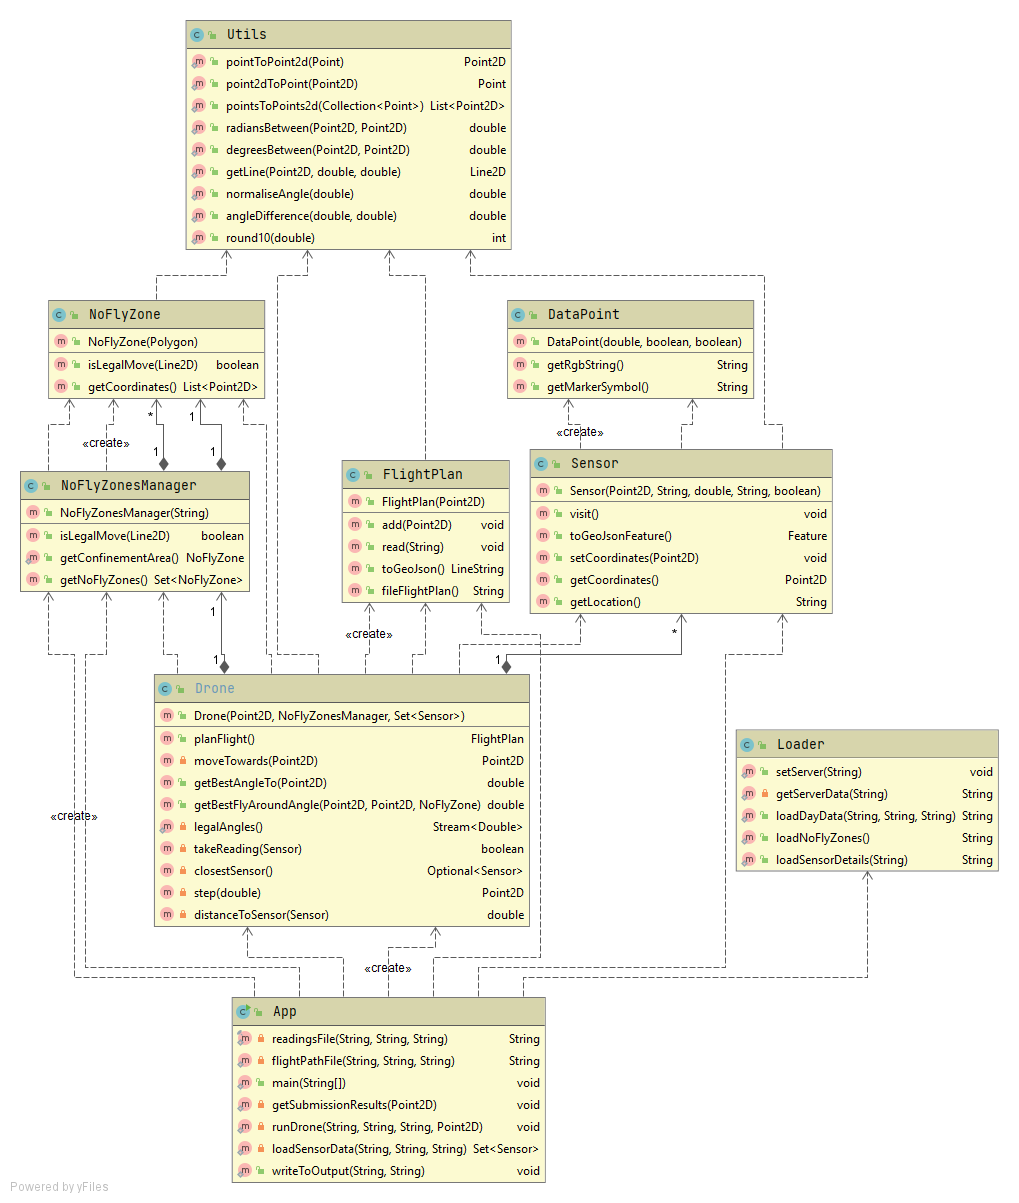
\includegraphics[scale=0.45]{cw2/ilp-report/Package aqmaps.png}
    \end{center}
\end{description} 

\pagebreak
%----------------------------------------------------------------------------------------
%	SECTION 2
%----------------------------------------------------------------------------------------

\section{Class Documentation}
This section will provide detailed documentation on all classes, methods and attributes. This also includes private methods, as this documentation is aimed for future maintainers of the project, which will need access to the whole structure and inner functioning.

\subsection{App.java}
\label{App.java}
This class is the entry point of the application. It provides methods to validate and parse the inputs, initialise a drone, and output its results. \\

\item[readingsFile()]
\texttt{private final String readingsFile(String day, String month, String year)}
Generates an appropriate readings filename for a given date.\\

\item[flightPathFile()]
\texttt{private final String flightPathFile(String day, String month, String year)}
Generates an appropriate flight path filename for a given date.\\

\item[main()]
\texttt{public static void main(String[] args)}
This is the entry point method. It handles inputs, startup the server (see \texttt{Loader}, and calls methods to run the drone.
It expects 7 arguments: day, month, year, initialLat, initialLng, serverPort and randomSeed. The random seed is not used (see drone implementation).

If started with the year \texttt{"0000"}, then it will generate all 24 submission files required in ilp-results. It handles exceptions when the network operations are interrupted.\\

\item[getSubmissionResults()]
\texttt{private static void getSubmissionResults(Point2D startingPoint)}\\
\texttt{throws IOException, InterruptedException}\\
Generates the $12\times2=24$ files required for the submissions. It runs a loop and generates a new \texttt{drone} for each required date. It throws IO exceptions when required. Those are handled in \texttt{main()}\\

\item[runDrone()]
\texttt{private static void}\\
\texttt{runDrone(String day, String month, String year, Point2D startingPoint)}\\
\texttt{throws IOException, InterruptedException}\\
Runs the \texttt{Drone} on a given date, starting at a given point. Throws the IO exceptions when required. In practice, is loads all necessary data from the server, start a Drone and call \texttt{Drone.planFlight()} to generate a \texttt{FlightPlan}, then calls \texttt{writeToOutput} to output the necessary files.\\


\item[runDrone()]
\texttt{private static Set<Sensor> loadSensorData(String day, String month, String year)}\\
\texttt{throws IOException, InterruptedException}\\
Uses the \texttt{Loader} class to make the necessary server requests. It takes a date to call the Loader, and returns a \texttt{Set<Sensor>} to be visited on that date. It also calls \texttt{Loader.loadSensorDetails} to populate the coordinates fields for each \texttt{Sensor}.\\

\item[runDrone()]
\texttt{private static void writeToOutput(String filename, String output)}\\
Writes the given \texttt{output} to a filename called \texttt{filename}, using a \texttt{PrintWriter}. Although it is a utility method, it belongs to the \texttt{App} class as it performs a major side effect. It catches all \texttt{FileNotFoundException}s and prints the output to console instead.\\


\subsection{DataPoint.java}
\label{DataPoint.java}
This class represents a single data point from a sensor. It contains static fields to define the appropriate marker colors and symbols for various readings and battery states. \\

\texttt{private final static int[] ranges}
This is an array of the upper bounds used to assign the colors and symbols.\\

\texttt{private final static String lowBatteryColor}\\
\texttt{private final static String notVisitedColor}\\
\texttt{private final static String[] readingColors}\\
\texttt{private final static String lowBatteryMarker}\\
\texttt{private final static String notVisitedMarker}\\
\texttt{private final static String[] readingMarkers}\\
These fields define the parameters given for the markers, with appropriate symbols and colors.\\

\texttt{private String rgbString}\\
\texttt{private String markerSymbol}\\
These fields represent Rgb color and marker symbol for the specific instance of a DataPoint. They are populated in the constructor.\\

\texttt{public DataPoint(double reading, boolean lowBattery, boolean visited)}
This is the main constructor of the class. It receives a reading and battery value, and a boolan to indicate if a sensor has been visited. It then assigns the appropriate color and marker according to what defined above.\\

\subsection{Drone.java}
\label{Drone.java}

This class represents a single Drone. It is a stateful drone (see algorithm later), aiming to visit all sensors, with the restrictions imposed by \texttt{NoFlyZonesManager}.\\

\texttt{private static final int ALLOWED\_NUMBER\_\OF\_MOVES = 150;}\\
\texttt{private static final double STEP\_LENGTH = 0.0003;}\\
\texttt{private static final double STEP\_ANGLE = 10;}/\\
\texttt{private static final double SENSOR\_RANGE = 0.0002;}\\
These fields define some given parameters for the drone. They are universal constants, therefore \texttt{static final}.\\

\texttt{private final Point2D startingPoint}\\
\texttt{private final NoFlyZonesManager noFlyZonesManager}\\
\texttt{private final HashSet<Sensor> sensors}\\
These fields represent instance variables. They are populated in the constructor. They are immutable references, therefore \texttt{final}\\

\texttt{private int movesLeft}\\
\texttt{private Point2D droneLocation}\\
These fields represent the actual state of the drone. They are mutable, and represent the number of moves left, and the actual drone location at any moment.\\


\texttt{public Drone(Point2D startingPoint,}\\
\texttt{\quad\quad NoFlyZonesManager noFlyZonesManager, Set<Sensor> sensors)}\\
This is the main constructor of the class. It receives a starting point, a no-fly-zones manager, and a Set of sensors to be visited. It does input validation and populates all local variables.\\

\texttt{public FlightPlan planFlight()}\\
Generates a valid \texttt{FlightPlan} for the drone, with requirements and restrictions given in the constructor. See Algorithm for details of the implementation.\\

\texttt{private Point2D moveTowards(Point2D targetDestination)}\\
Make a move towards the target destination. Calls \texttt{getBestAngleTo} to get an appropriate valid angle. Returns a \texttt{Point2D} representing the drone location after the move.\\

\texttt{private double getBestAngleTo(Point2D targetDestination)}\\
Get the best \textbf{legal} angle to go to the target destination. This is not always the straight-line angle, such as when there is a no-fly-zone in the path, or if the angle is not legal for the drone to fly.\\

\texttt{private double getBestFlyAroundAngle(Point2D start,}\\
\texttt{\quad\quad Point2D targetDestination, NoFlyZone noFlyZone)}\\
Get the best \textbf{legal} angle to \textbf{fully} fly around a given \texttt{NoFlyZone}. It returns the closest angle to a straight-line path, that never intersects the no-fly-zone. This assures the least number of moves is used to fly around it. See algorithm for implementation.\\

\texttt{private static Stream<Double> legalAngles()}\\
Generates a Stream of all legal angles for the drone to fly. This is generalised on \texttt{STEP\_ANGLE}; in this case it returns all multiples of $10$ up to \textemdash but excluding \textemdash $360$.\\

\texttt{private boolean takeReading(Sensor sensor)}\\
Tries to take a reading of a sensor. Returns whether the reading succeeded (i.e.: the sensor was in range).\\

\texttt{private Optional<Sensor> closestSensor()}\\
Returns the optional closest sensor to the drone. If no sensor exist, it returns \texttt{Optional.empty()}.\\

\texttt{private Point2D step(double radians)}\\
Makes one step of \texttt{STEP\_LENGTH} in the specified direction. No side effect is performed, but the resulting position is returned.\\

\texttt{private double distanceToSensor(Sensor sensor)}\\
Finds the distance to a sensor.\\


\subsection{FlightPlan.java}
\label{FlightPlan.java}

This class represents a full flight plan. It makes use of an inner class to represent a single component (i.e. step) in the plan. It provides methods to help generate maps as a result. It uses a \texttt{Deque} to represent the flight plan, as this is an efficient data structure when operating on the ends only. \\

\texttt{private final Point2D startingPoint}\\
\texttt{private final Deque<FlightPlanComponent> flightPlan}\\
These fields represent instance attributes.\\

\texttt{public FlightPlan(Point2D startingPoint)}
This is the main constructor of the class. It takes a starting point, and initialises the fields appropriately.\\

\texttt{public void add(Point2D point)}
Adds a destination point to a flight plan. Generates the angle based on the previous location.\\

\texttt{public void read(String sensorLocation)}
Add the reading of a sensor to the flight plan.\\

\texttt{public LineString toGeoJson()}
Generates a GeoJson LineString representing the FlightPlan.\\

\texttt{public String fileFlightPlan()}
Generates a String representing the FlightPlan. This is a format according to \texttt{FlightPlanComponent.toString}.\\
\subsection{FlightPlanComponent.java}
\label{FlightPlanComponent.java}
This class represents a single entry in flight plan. It has all the informations needed to fill a flightpath file according to specification. \\

\texttt{public Point2D getEnd()}
Returns the destination of the move.\\

\texttt{public String toString()}
Generates a String representation of the component, according to specification.\\

\subsection{Loader.java}
\label{Loader.java}
This class is responsible for the loading of the network resources. It does not do any processing of the data nor exception handling. It uses static methods as network resources are expendive. This way, only one client is created. \\\\

\texttt{private static final String dayDataFilename = "air-quality-data.json";}\\
\texttt{private static final String noFlightZonesFilename = "no-fly-zones.geojson";}\\
\texttt{private static final String sensorLocationFilename = "details.json";}\\
Filenames constants.\\

\texttt{public static void setServer(String server)}
Sets the server to be used for the API calls. Should include protocol, address and port. E.g: \texttt{Loader.setServer("https://localhost:8080")}.\\

\texttt{private static String getServerData(String path)}\\
\texttt{throws IOException, InterruptedException}\\
Method to make a network request for a resource at the given path, in the set server. Throws exceptions if the IO operation fails.\\

\texttt{public static String loadDayData(String day, String month, String year)}\\
\texttt{throws IOException, InterruptedException}\\
Method to load the daily list of sensors.\\

\texttt{public static String loadNoFlyZones()}\\
\texttt{throws IOException, InterruptedException}\\
Method to load buildings data.\\

\texttt{public static String loadSensorDetails(String location)}\\
\texttt{throws IOException, InterruptedException}\\
Method to load a sensor detail, given a What3Words location for it.\\


\subsection{NoFlyZone.java}
\label{NoFlyZone.java}
This class represents a single no-fly-zone. It is represented a List of Line2D. \\

\texttt{private final List<Point2D> coordinates}\\
\texttt{private final List<Line2D> boundaries}\\

\texttt{public NoFlyZone(Polygon polygon)}
Class constructor. Generates a NoFlyZone from a valid GeoJson \texttt{Polygon}.\\

\texttt{public boolean isLegalMove(Line2D move)}\\
Checks if a Line2D move is legal (i.e. does not intersect any zone boundary).\\

\texttt{public List<Point2D> getCoordinates()}\\

\subsection{NoFlyZonesManager.java}
\label{NoFlyZonesManager.java}
This class manages the \texttt{NoFlyZones}. It is in fact a map authority. It includes the confinement area. \\

\texttt{private static final NoFlyZone confinementArea}\\

\texttt{private final Set<NoFlyZone> zones}
The Set of no-fly-zones that this instance contains.\\

\texttt{public NoFlyZonesManager(String geoJson)}\\
Class constructor. It inisialises the no-fly-zones from a GeoJson \texttt{Polygon} array.\\

\texttt{public boolean isLegalMove(Line2D move)}\\
Checks if a Line2D move is legal (i.e. does not intersect any no-fly-zone).\\


\texttt{public static NoFlyZone getConfinementArea()}\\

\subsection{Sensor.java}
\label{Sensor.java}
This class represents a single Sensor. It includes methods to visit it, as well as to generate a GeoJson marker representation of it. It uses \texttt{DataPoint} to do this. \\

\texttt{private Point2D coordinates;} \quad The coordinates location of the sensor.\\
\texttt{private final String location;} \quad The What3Words location of the sensor.\\
\texttt{private final double battery;}\\
\texttt{private final String reading;}\\
\texttt{private boolean visited;}\\

\texttt{public Sensor(Point2D coordinates, String location,}\\
\texttt{\quad\quad double battery, String reading, boolean visited)}\\
The Class constructor. It is never used as the sensors are generated by \texttt{Gson}\\

\texttt{public void visit()}\\
Method to mark this sensor as visited.\\

\texttt{public Feature toGeoJsonFeature()}\\
This method returns a GeoJson \texttt{Feature} representing this sensor. It uses \texttt{DataPoint} to get the appropriate color and marker symbol.\\

\texttt{public Point2D getCoordinates()}\\
\texttt{public void setCoordinates(Point2D coordinates)}\\
\texttt{public String getLocation()}\\

\subsection{Utils.java}
\label{Utils.java}
This class contains a collection of static utility methods. They mostly deal with data types conversion and trigonometry functions. \\

\texttt{public static Point2D pointToPoint2d(Point point)} \quad Converts a Point to Point2D.

\texttt{public static Point point2dToPoint(Point2D point2d)} \quad Converts a Point2D to Point.\\

\texttt{public static List<Point2D> pointsToPoints2d(Collection<Point> points)}\\ Convert a Collection of Point2D to a List of Point.\\

\texttt{public static double radiansBetween(Point2D point1, Point2D point2)}\\
Find the \textbf{positive} angle that a line segment from \texttt{point1} to \texttt{point2} makes with the positive X axis.\\

\texttt{public static double degreesBetween(Point2D point1, Point2D point2)}\\
Find the \textbf{positive} angle that a line segment from \texttt{point1} to \texttt{point2} makes with the positive X axis.\\

\texttt{public static Line2D getLine(Point2D start, double degrees, double length)}\\
Calculates the Line2D starting from a point, with a given angle in degrees and a given length.\\

\texttt{public static double normaliseAngle(double degrees)} \quad Map an angle to the range $[0, 360)$.\\

\texttt{public static double angleDifference(double angle1, double angle2)}\\
Find the \textbf{normalised} difference between two angles (i.e: in $[0, 360)$).\\

\texttt{public static int round10(double degrees)} \quad Round an angle to the nearest multiple of 10.\\

\pagebreak
%----------------------------------------------------------------------------------------
%	SECTION 3
%----------------------------------------------------------------------------------------

\section{Drone control algorithm}

\subsection{Brief description of the drone}
The Drone has full knowledge of the sensors location and which ones have been visited. The handling of no-fly-zones is partially delegated to the \texttt{NoFlyZonesManager}, which determines if a move is legal to make. Here is a brief pseudocode representing the algorithm.


\begin{verbatim}
    while there are moves left:
        target = closest sensor OR starting point (see 3.6)
        find the angle to go there
            if it intersects a no-fly-zone
                fly around it
            else
                round the angle to 10 and go there
        if close to the sensor
            read it
        moves -= 1
\end{verbatim}

\subsection{Prioritization problems}
The first problem that the drone encounters, is a prioritization problems. It has to choose which sensor to head to at each step, and move there. This implementation of the drone follows a simple Greedy Algorithm. This is a type of algorithm that "follows the problem-solving heuristic of making the locally optimal choice at each stage"\cite{wiki:greediAlgo}. In this case, the optimal choice aims to minimise the euclidean distance from the drone to the sensor:
\begin{align*}
    distance = \sqrt{(\text{drone.X} - \text{sensor.X})^2 + (\text{drone.Y} - \text{sensor.Y})^2}.
\end{align*}
It uses the \texttt{Collections.min} and \texttt{Point2D.distance} methods for this.

In other words, it just tried to go to the closest sensor as the crow (drone) flies.
Although this does not take no-fly-zones into account, it can provide a solution to the prioritization problems in linear time $O(n)$ to the number of sensors left to visit. 

\subsection{NoFlyZones}
Once it finds the sensors it'd like to go to, the optimal move would be to move from its location to the sensor. Let us call this line segment \textit{straightLine}. The first thing to do, is to check if this line intersects any no-fly-zone. Those are provided by a \texttt{NoFlyZonesManager}. If there is a no-fly-zone in the straightLine, then we use \texttt{getBestFlyAroundAngle} to fly around it. Otherwise, we attempt to make a move. We legalise the straightLine angle by round it to 10, and make a move of \texttt{STEP\_LENGTH}. We validate this move against the no-fly-zones, and make it. If this new rounded angle crashes a no-fly-zone, use the same \texttt{getBestFlyAroundAngle} to legalise it. We check for both the full-length line and a step-length line to ensure we are not just going towards a no-fly-zone, just to have to fly around it later. See the next section for more details. This is a pseudo-code for this:

\begin{verbatim}
    function getBestAngleTo(destination):
        straightLine = the straight line
        validMove = straight line move, with rounded angle and 1 step length
        for each no-fly-zone:
            if not legal(straightLine) or not legal (validMove)
                move = getBestFlyAroundAngle()
        return validMove
\end{verbatim}

\subsection{getBestFlyAroundAngle}
When there is a no-fly-zone in the path from the drone to a sensor, no matter how far, it is not efficient to just move forward and turn just before hitting it. This is what the \texttt{getBestFlyAroundAngle} function ensures.

Given a destination and a \texttt{NoFlyZone}, it returns a valid angle that never intersects the zone. This ensures a full fly around is possible. Not only this, but the angle is guaranteed to be the closest one to the straightLine we identified earlier. These two facts, ensure we can fly around a no-fly-zone to reach a destination, in the quickest way possible. Let us imagine a drone trying to go from point A to point B. A naive drone would follow the black path, reach the library no-fly-zone, and turn around it. However, a drone with full knowledge, is able to see the library, and have an optimal path to fly around it as soon as possible:

\begin{center}
    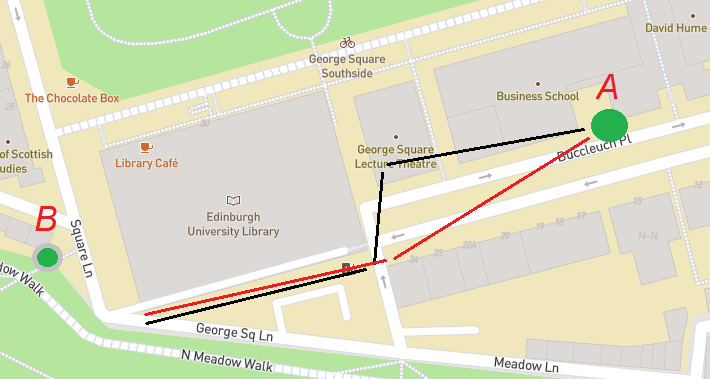
\includegraphics[scale=0.7]{cw2/ilp-report/algo.png}
\end{center}

Here is how the algorithm works:

\begin{verbatim}
    function getBestFlyAroundAngle(destination, zone):
        angles = getValidAngles (helper function to get all multiples of 10 up to 360)
        for each angle in angles:
            line = line starting at the drone, at that angle and infinite length
            if line intersects zone:
                remove angle from angles
        filter out the angles that in a STEP_LENGTH intersect any zone
        get the angle with the lowest deviation from the straightLine
        move in that direction
\end{verbatim}

In fact, an exception is made for the confinement area. As mentioned earlier, this is represented as a no-fly-zone, as the drone is not allowed to cross it. However, as the drone is inside, it'll never be able to fully fly around it. Therefore, if the drone crashes with the confinement area, it'll skip the for-loop check and just filter out
based on the next \texttt{STEP\_LENGTH}.

In practice, this whole operation is achieved through \texttt{Stream}s: \texttt{Stream.filter()} and \texttt{Stream.min()} are used. This insures optimal performance.


\subsection{Reading a sensor}
Finally, at every move we try to read the closest sensor. If this read is successful (the sensor is in range), we mark its object as read, and remove it from the list of sensors to be visited.

Otherwise, we decrease the number of moves left, and repeat the loop. At every move, we recalculate the closest sensor, as it may be the case that, while flying around a no-fly-zone, we got very close to another sensor, so it is preferred to read that one first, and then keep flying around the zone.

\subsection{Going back to the starting point}
Once all sensors have been visited, the result of \texttt{getClosestSensor()} would be an empty object. Consequently, we set the target destination as the starting point, and follow the same process to get there avoiding the no-fly-zones.

\subsection{Results}
Once a \texttt{FlightPath} object is generated by the drone, we call its \texttt{toString} method to get a flightpath and save it to file. Similarly, its \texttt{toGeoJson} method is used to generate a \texttt{LineString} to plot a map. Here is the output of the drone generated on two different days:

\begin{center}
    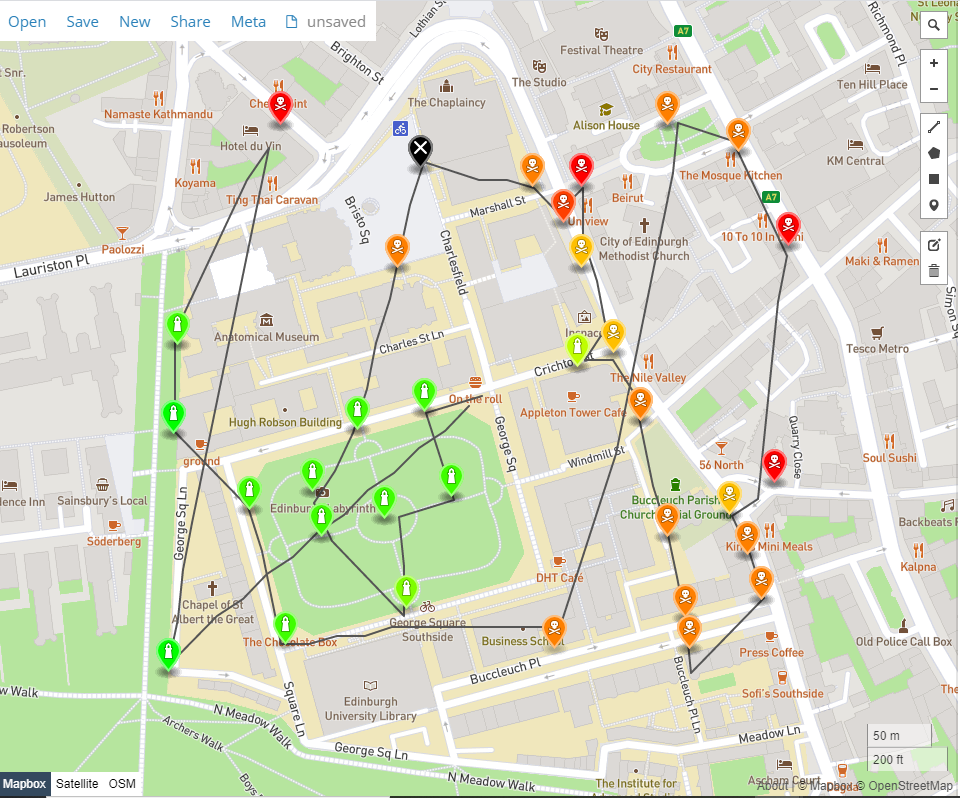
\includegraphics[scale=0.65]{cw2/ilp-report/res1.png}\\
    Drone output path for the date 01/01/2020
\end{center}

In this graphic, we can clearly see the drone starting in the middle of the map. It then follows a path of sensors around the meadows, then in the top part and around Nicolson street, just to finish those left in the meadows and go back to the starting point.

We can clearly see the fly-around of Appleton Tower, as well as a slight one around the library

\begin{center}
    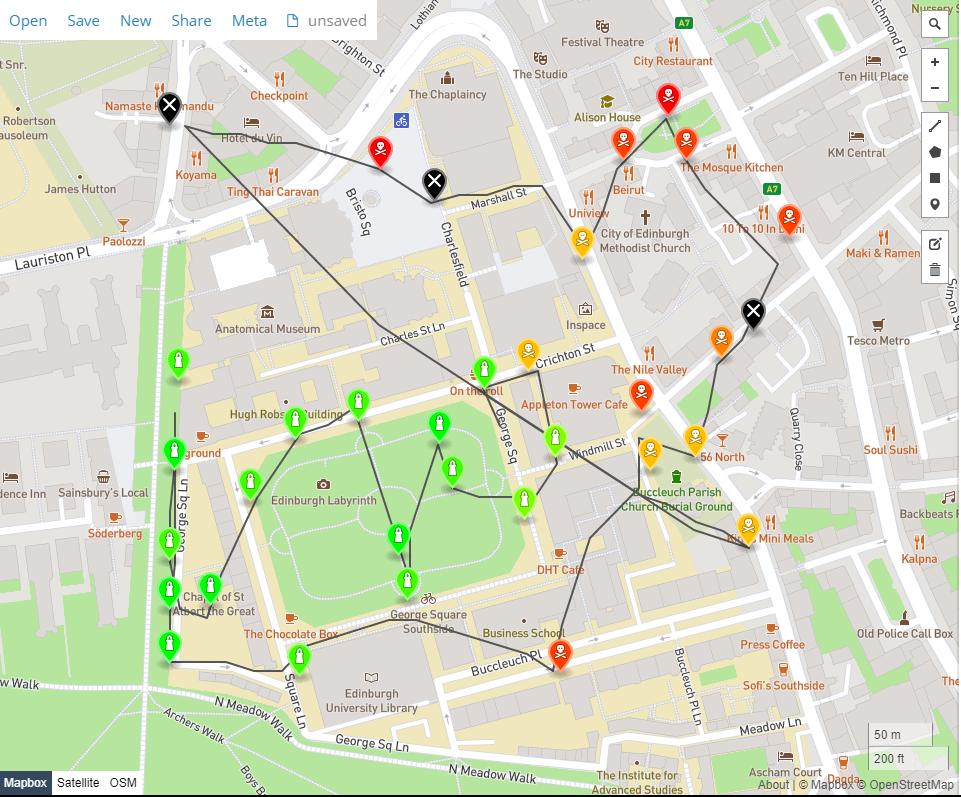
\includegraphics[scale=0.65]{cw2/ilp-report/res2.png}\\
    Drone output path for the date 12/12/2020
\end{center}
Similarly here, the drone starts in the middle, reads the sensors around 50 George Square and those in the meadows. It then heads to Nicolson street, up to the Mosque Kitchen and finishes reading the ones left, to then head back to the starting point.

Additionally, we can clearly see how it flies around the Library to reach a sensor.


\subsection{Testing}
The application has been thoroughly tested for functionality. Assertions are provided when appropriate.

%----------------------------------------------------------------------------------------
%	BIBLIOGRAPHY
%----------------------------------------------------------------------------------------

\bibliographystyle{unsrt}

\bibliography{bib}

%----------------------------------------------------------------------------------------


\end{document}